\begin{figure}[t]
  \centering
  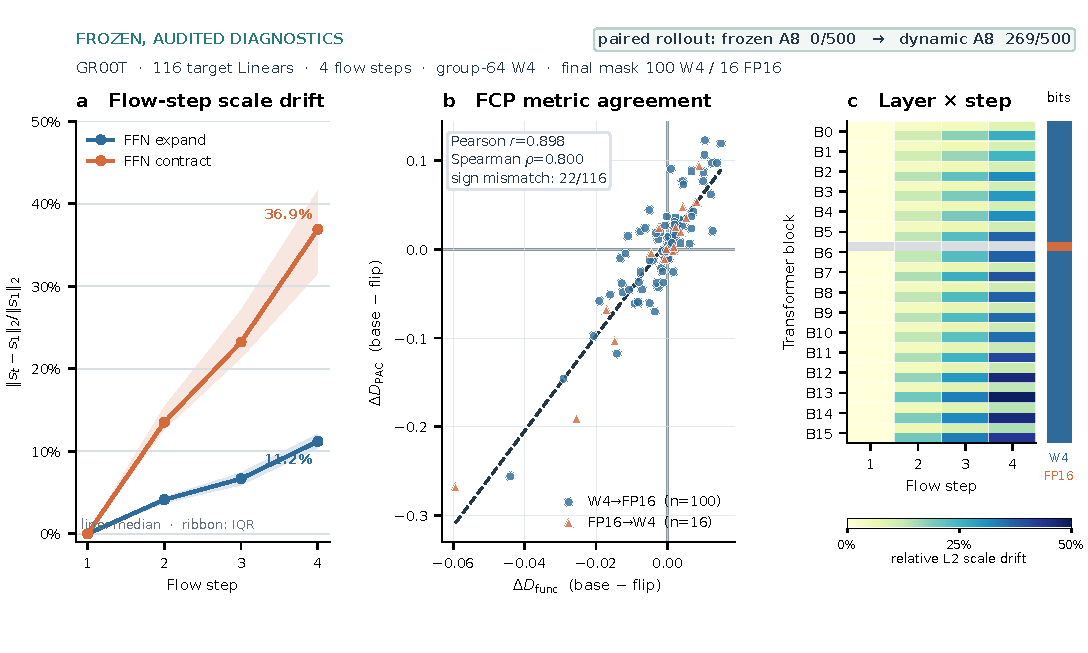
\includegraphics[width=\textwidth]{figures/dypac_quantization_diagnostics.pdf}
  \caption{Audited quantization diagnostics. \textbf{(a)} The relative $\ell_2$ drift of each frozen per-channel A8 scale vector from flow step 1; lines and ribbons show the median and interquartile range over W4 action-head layers. The paired rollout badge reports the frozen-range and deployed dynamic-A8 outcomes. \textbf{(b)} Changes in \dfunc and \dpac for all 116 one-layer full-context counterfactuals; positive values favor the flipped mask, and the dashed line is an ordinary least-squares guide. \textbf{(c)} The same scale drift for both FFN targets in each action-head transformer block. Gray denotes the protected FP16 row, for which no A8 table is applied. The plotted frozen ranges are diagnostic ablation artifacts, not deployment-time lookup tables.}
  \label{fig:quantization_diagnostics}
\end{figure}
